% TeX root=../main.tex

\section{Concordância}

Adjetivos concordam em gênero, número e caso com seu
substantivo.
Adjetivos modificando um possessor expresso por um adjetivo de posse em
\emph{-asi-} concordam com o adjetivo de posse:

\exg. \emph{wasu-s} \emph{Runtiy-asi-s} \emph{nimuwiza-s}\\
bom-\Nom\Sg\Com{} R.-\emph{poss.}-\Nom\Sg\Com{} filho-\Nom{}\Sg\Com{}\\
o filho do bom Runtiya \emph{ou} bom filho de Runtiya


\noindent Verbos concordam com o sujeito em número e pessoa.

Verbos com seu sujeito no neutro plural podem permanecer no singular:

\exg.\emph{katin-a} \emph{wasuw-a} \emph{as-ti}\\
vasilha-\Nom\Pl\Neut{} bom-\Nom\Pl\Neut{} ser-3\Sg\textsc{Ind.Pres.}\\
as vasilhas são boas


\noindent Numerais acima de um podem modificar substantivos no singular.


\section{Uso dos casos}

\paragraph{Nominativo}
Caso do sujeito e predicativo do sujeito.
Orações predicativas na maioria das vezes não utilizam o verbo \emph{as-} `ser'.

\exg.\emph{katin-a} \emph{wasuw-a} (\emph{as-ti})\\
vasilha-\Nom\Pl\Neut{} bom-\Nom\Pl\Neut{} (ser-3\Sg\textsc{Ind.Pres.})\\
as vasilhas são boas


\paragraph{Acusativo}
Expressa normalmente o objeto direto da oração.
Outros usos incluem:
\begin{inparaenum}[(a)]
	\item duplo acusativo: \emph{amu=pa=wa=\textbf{n} zadi \textbf{istran} daha}
		`aqui eu \textbf{o} peguei \textbf{pela mão}' (KARKAMIŠ A7, §3).
	\item duração de tempo: \emph{\logo{`ANNUS'}-an \logo{ANNUS}-an} `ano após
		ano'.
\end{inparaenum}


\paragraph{Genitivo}
Expressa posse e pode ser substituído pelo adjetivo de posse em \emph{-asi-} e a
pluralidade apenas pode ser entendida a partir do adjetivo de posse:

\ex.\ag.\emph{tati-s} \emph{masan-inzi}\\
pai-\Gen\Sg\Com{} deus-\Nom\Pl\Com{}\\
os deuses do pai 
\bg.\emph{tat-as-inzi} \emph{masan-inzi}\\
pai-\emph{poss.}-\Nom\Pl\Com{} deus-\Nom\Pl\Com{}\\
os deuses dos pais\slash{}do pai\slash{}paternos


\paragraph{Dativo--Locativo}
Expressa tanto o objeto indireto do verbo quanto o local em que a ação verbal
ocorre. Outros valores semânticos podem ser expressos pelo dativo:
\begin{inparaenum}[(a)]
\item dativo de posse\slash{}interesse: \emph{a=wa=\textbf{ti} alamanza izisatai} `ele
	honra o nome \textbf{para si} $\rightarrow$ ele honra \textbf{seu próprio} nome';
\item  direção\slash{}alativo;
\item dativo de comparação;
\item tempo em que algo ocorre: \emph{apadi \logo{ANNUS}-usi} `naquele ano';
\item objeto de infinitivos (raro).
\end{inparaenum}


\paragraph{Ablativo--Instrumental}
Expressa lugar de origem de um movimento, separação ou instrumento de uma ação.
Outros usos incluem:
\begin{inparaenum}[(a)]
\item causa de um evento;
\item agente da passiva: \emph{\textbf{masanadi} azamis hantawatis} `rei amado 
	\textbf{pelos deuses}'.
\end{inparaenum}


\section{Comparação}
Pode ser expressa por dois dispositivos sintáticos:
\begin{compactenum}[(a)]
\item adjetivos seguindo \emph{\logo{FRONS}-li- = hantili-} `o mais X':\\
	\emph{hantili \logo{ARGENTUM.DARE}-siya} `o mais caro'.
\item N$_{1,i}$ N$_{2,\emph{dat.}}$ Adj.$_i$ `N$_1$ é mais Adj.\ que N$_2$':\\
	\emph{apas=wa=mu \textnormal{(N$_1$)} lananza \textnormal{(N$_{2,dat.}$)} uran
	\textnormal{(Adj)} izida}\\
	`ele me (N$_1$) fez maior (Adj) que os irmãos (N$_{2,dat.}$)';
\end{compactenum}

\section{Advérbios}
\lipsum[1-2]

\section{Posposições}

\section{Pronomes}

\section{Ordem de palavras}

\section{Interrogações}

\section{Coordenação}

\section{Subordinação}

\paragraph{Causais}

\paragraph{Condicionais}

\paragraph{Concessivas}

\paragraph{Consecutivas}

\paragraph{Relativas}

\paragraph{Temporais}



\chapter{Leitura: BOHÇA}


% \begin{center}
% 	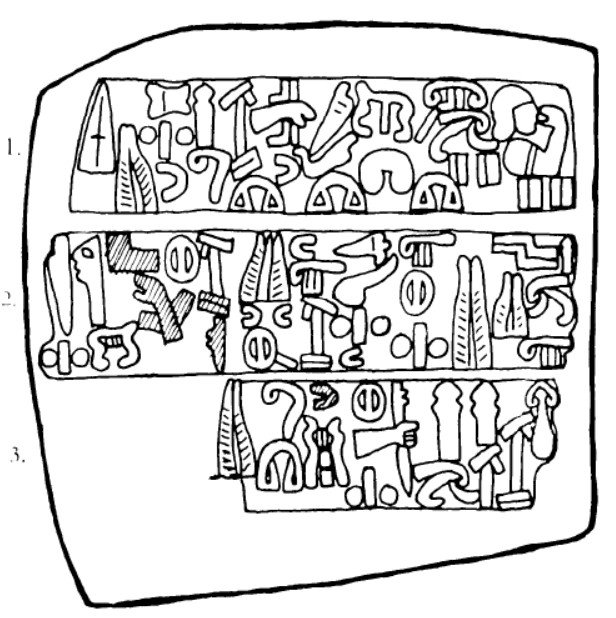
\includegraphics[width=0.85\textwidth]{../../../Mídia/hama14.jpg}
% \end{center}


\begin{parnumbersa}[]
	\raggedright%

	\Large \luwiantrans{EGO-mi}\hspace{5pt}
	\luwiantrans{ku-ra-ti-i-sá}\hspace{5pt}
	\luwiantrans{á-[sa-hwi-si]-sa4}\hspace{5pt}
	\luwiantrans{HEROS-li-i-sa}\hspace{5pt}
	\luwiantrans{<FILIUS>-ni-mu-wi-za-sa}\hspace{5pt}
	\luwiantrans{REX}


	\Large \luwiantrans{a-wa}\hspace{5pt}
	\luwiantrans{á-mu}\hspace{5pt}
	\luwiantrans{AEDIFICARE-mi-ha}\hspace{5pt}
	\luwiantrans{za-a}\hspace{5pt}
	\luwiantrans{<CASTRUM>-hara-ni-sà-za}\hspace{5pt}
	\luwiantrans{la-ka-wa-ni-sà-ha-wa REGIO}\hspace{5pt}
	\luwiantrans{FLUMEN-REGIO-da-i-sà}

	\Large \luwiantrans{REL-za} \hspace{5pt}
	\luwiantrans{i-zi-i-da}\hspace{5pt}
	\luwiantrans{a-tá-ha-wa}\hspace{5pt}
	\luwiantrans{ni-ki-ma-sa REGIO}

\end{parnumbersa}

\vspace{10pt}
\hrule
\vspace{10pt}

\setcounter{parcount}{0}
\begin{parnumbersa}[]

	\raggedright%
	\itshape%

	\logo{EGO}-mi
	\logo{MAGNUS}+ra/i-da-mi-sa
	u-ra/i-hi-li-na-sa
	\logo{FILIUS}.NI-za-sa
	i-ma-tú-wa/i-ni\logo{(REGIO)} \logo{REX}

	a-wa/i á-mu \logo{AEDIFICARE}+MI-ha za-' \logo{(``CASTRUM'')}hara/i-ni-sà-za
	la-ka-wa/i-ni-sà-ha-wa/i\logo{(REGIO)} \logo{FLUMEN.REGIO}-da-i-sà

	\logo{REL}-za i-zi-i-da a-tá-ha-wa/i ni-ki-ma-sa\logo{(REGIO)}


\end{parnumbersa}

\vspace{10pt}
\hrule
\vspace{10pt}


\setcounter{parcount}{0}
\begin{parnumbersa}[]

	\raggedright%
	\itshape%
	amu=mi Uradamis Urhilinas nimuwizas imatuwani hantawatis.

	a=wa amu tamaha za harnisa=za, lakawanis hapadis

	kwa=za izida, anta=ha=wa Nikimas.


\end{parnumbersa}

\vspace{10pt}
\hrule
\vspace{20pt}


\clearpage%

\ex.[]\ag.[1] \emph{amu} \emph{=mi} \emph{Uradamis} \emph{Urhilinas}
\emph{nimuwizas} \emph{imatuwani} \emph{hantawatis.}\\
\Pro{}1\Sg{} =\Refl{}. U.-\Com{}\Nom{}\Sg{} U.-\Com{}\Gen{}\Sg{} filho-\Com{}\Nom{}\Sg{}
imatuano-\Com{}\Nom{}\Sg{} rei-\Com{}\Nom{}\Sg{}\\
Eu sou Uradamis, filho de Urhilinas, rei imatuano.
\bg.[2] \emph{a} \emph{=wa} \emph{amu} \emph{tamaha} \emph{za} \emph{harnisa=za,}\\
\Conj{} =\Clt{} \Pro{}1\Sg{} construir-1\Sg{}\Pret{} \Pro{}\Neut{}\Acu{}\Sg{}
fortaleza-\Neut{}\Acu{}\Sg{}=\Clt{}\\
E eu (mesmo) construí esta fortaleza,
\bg.[||] lakawanis =ha =wa hapadis\\
L.\Com{}\Nom{}\Sg{} =\Conj{} =\Clt{} fluvial-\Com{}\Nom{}\Sg{}\\
\bg.[3] \emph{kwa=za} \emph{izida},\\
\Rel{}\Neut{}\Acu{}\Sg{}=\Clt{} fazer-3\Sg{}\Pret{}\\
a qual o povo de Laka fez,
\bg.[] \emph{anda=ha=wa} \emph{Nikimas}.\\
dento=\Conj{}=\Clt{} N.\Com{}\Nom{}\Sg{}\\
E dentro [dela está] Nikima.



\bigskip
\begin{multicols}{2}[\noindent\textbf{Vocabulário}]
	\begin{hangparas}{1em}{1}
		\raggedright%
		\textbf{\emph{amu}} (\emph{pron.1sg.}) \tabto{1em} eu\\
		\textbf{\emph{anda}} (\emph{adv.}) \tabto{1em} dentro\\
		\textbf{\emph{halpa}-} (TO) \tabto{1em} Halpa\\
		\textbf{\emph{halpawani}-} (\emph{adj.}) \tabto{1em} proveniente de Halpa \tabto{1em} halabeu\\
		\textbf{\emph{hantawati}-} (\emph{subst.com.}) \tabto{1em} rei\\
		\textbf{\emph{hapadi}-} (\emph{adj.}) \tabto{1em} fluvial\\
		\textbf{\emph{harnisa}-} (\emph{subst.neut.}) \tabto{1em} fortaleza\\
		\textbf{\emph{imatuwani}-} (\emph{adj.}) \tabto{1em} proveniente de Hama
		\tabto{1em} imatuano\\
		\columnbreak%
		\textbf{\emph{izi{(ya)}}-} (\emph{v.t.}) \tabto{1em} fazer, criar\\
		\textbf{\emph{lakawani}-} (\emph{adj.}) \tabto{1em} proveniente de Laka\\
		\textbf{\emph{nikima}-} (TO) \tabto{1em} Nikima\\
		\textbf{\emph{nimuwiza}-} (\emph{subst.com.}) \tabto{1em} filho\\
		\textbf{\emph{tama}-} (\emph{v.t.}) \tabto{1em} construir\\
		\textbf{\emph{Uradami}-} (NP) \tabto{1em} Uradamis\\
		\textbf{\emph{Urhilina}-} (NP) \tabto{1em} Urhilina\\
	\end{hangparas}
\end{multicols}

\clearpage
\subsubsection*{Notas}

\paragraph{Linha 1}
\textbf{amu=mi} `eu (sou)': o verbo \emph{as-} `ser, estar' é com frequência deixado
explícito em sentenças nominais e nestes casos costuma-se utilizar a
forma reflexiva do pronome.

\noindent\textbf{imatuwani} `imatuano, proveniente de Hama': em casos muito raros, a
desinência do nominativo singular comum não é expressa na grafia, algo que é
mais comum em inscrições majoritariamente logográficas. A série de inscrições de
Uradamis em Hama (1--3 e 6--7) não utilizam a desinência no gentílico
\emph{imatuwani-}.
Curiosamente, as inscrições de Urhilina, pai de Uradamis, HAMA 4,
RESTAN, QAL\textsc{ʿ}AT EL MUDIQ e HINES,
também não empregam desinência de nominativo no gentílico e, em adição, não
incluem a desinência no nome próprio do rei.
HAMA 8, no entanto, também de Urhilina, emprega a desinência no gentílico, mas
não no nome do rei.
Algumas outras inscrições escavadas em Hama, a saber, MEHARDE e SHEIZAR, empregam
regularmente as desinências.

\noindent\textbf{nimuwizas} `filho': por vezes, assume-se a existência de \emph{niza-}
`filho', um sinônimo de \emph{nimuwiza-} `filho', mas atualmente entende-se que
a grafia <FILIUS-ni-za-sa> e similares representa o logogram FILIUS com o
complemento fonológico \emph{NI} e /za-sa/ representem a fonologia da forma
subjacente, daí que transliteramos FILIUS.\emph{NI}-za-sa
(\citeabbrev*{CHLI3} \emph{ad loc.}).

\noindent\luwiantrans{REX} \textbf{= hantawatis} `rei': a forma sempre é escrita com \luwiantrans{REX} e
nunca é escrita com sua fonologia completa,
apenas com o final \emph{ti-}.\footnote{Raríssimas vezes, com \emph{-ta-}.}
Reconstrói-se a forma subjacente a partir do luvita cuneiforme
\emph{handawati-} `rei'.

\paragraph{Linha 2}
\textbf{amu} `eu': quando o pronome pessoal é utilizado, costuma-se entender que
seja para denotar algum tipo de ênfase, algo como `eu mesmo, fui eu que\ldots{}'.

\noindent\luwiantrans{AEDIFICARE-mi-ha} \textbf{= tamaha} `(eu) construí': note no
traçado da inscrição que \luwiantrans{mi} está \emph{em volta} da mão do
logograma \luwiantrans{AEDIFICARE}. Este uso é frequente para indicar que a
forma subjacente de um certo logograma contém em alguma parte de seu tema um
fonema /m/, independentemente do valor da vogal.\footnote{Por vezes, além
	do complemento fonológico anexado ao logograma, a sílaba /ma/ é representada
	por silabogramas: AEDIFICARE.\emph{MI}-ma-da = \emph{tamada} `ele construiu'
	(KARATEPE 2, §1).}

\noindent\luwiantrans{za-a} \textbf{= za' = za}: o sinal L.450 \luwiantrans{a} funciona
aqui de espaçador.
\textbf{harnisa=za}: \emph{=za} como partícula de dupla marcação do acusativo
neutro singular.

\paragraph{Linhas 2-3}
\textbf{la-ka-wa/i-nis=ha=wa/i REGIO} `povo de Laka': notar que o logograma
determinativo aparece no \emph{final} da escrita fonológica e após a cadeia de
clíticos.

\noindent\luwiantrans{FLUMEN.REGIO-da-i-sà} \textbf{= hapadis} `[terra] fluvial;
alagadiço': nas inscrições HAMA 1--3, parece que os escribas imatuanos,
para deixarem claro que uma sílaba /Ti/ contém uma oclusiva sonora /d/,
escrevem a sequência \luwiantrans{da-i} <da-i> ao invés de empregarem o
silabograma \luwiantrans{ti} <ti>, que poderia representar tanto /ti/ quanto
/di/. No resto do \emph{corpus}, a forma é regularmente escrita com
\luwiantrans{ti} <ti>.\footnote{
	Para uma interpretação contrária, ver~\citet{Simon2019}, que propõe que o
	sinal L.41 possa ter também o vocalismo em /i/, assim <da/i>.
}

\noindent\textbf{lakawanis\ldots{} hapadis} `povo da terra fluvial de Laka': sujeito da
oração relativa iniciada na linha seguinte por \emph{kwa{(n)}=za}.
O motivo da prolepse é incerto, mas pode-se argumentar que a troca de
sujeito\slash{}tópico de Uradamis para o povo de Laka a tenha motivado.

\noindent\textbf{kwa{(n)}=za} `a qual': o referente da relativa é \emph{harnisa=za}
[2].

\noindent\textbf{izida} `fez': o contraste feito entre \emph{amu tamaha} `eu (mesmo)
construí' e \emph{lakawanis hapadis kwa{(n)}=za izida} `o povo da região
fluvial de Laka que a fez' é bastante marcado tanto pela presença do pronome
pessoal quanto pela prolepse do sujeito da oração relativa.
O mesmo ocorre em todas as outras inscrições HAMA 1--3 e 6--7:
\begin{compactitem}
	\item HAMA 1: \emph{hurpadawanis hapadis kwa=za izida} `a qual o povo da região
	fluvial de Hurpada fez'
	\item HAMA 3: \emph{musanipawanis hapadis kwa=za izida} `a qual o povo da região
	fluvial de Musanipa fez'
	\item HAMA 6: \emph{kusunalanzi kwa=za iziyanta} `a qual os kussunalitas fizeram'
	\item HAMA 7: MONS \emph{labarnawanis hapadis kwa=za izida} `a qual o
	povo da região fluvial do monte Labarna fez'
\end{compactitem}

\noindent\textbf{anda=ha=wa} `e dentro [está]': as inscrições HAMA 1, 2 e 7
terminam com esta fórmula seguida de um topônimo.
A fortaleza não poderia cobrir a extensão necessária para conter todos os
territórios nomeados, de modo que se a interpretação for literal `dentro da
fortaleza está X', deve-se entender `dentro está parte da população de X',
talvez aquartelada para defender a fortaleza.
Outra interpretação possível é que em 1, 2 e 7, estejam sendo adicionados outros
povos à lista dos que fizeram, com o sentido `fortaleza a qual o povo Y fez,
\emph{incluindo} o povo de X'.


\begin{flushleft}
	\noindent \textbf{Tradução}\\
	\noindent [1] ``Eu sou Uradamis, filho de Urhilina, rei imatuano. [2] Eu mesmo
	construí esta fortaleza, (e) o povo de Laka, região fluvial, [3] que a fez e
	dentro está Nikima
\end{flushleft}

